\section{Approach Overview}
\label{overview:sec}

{\tool} has two main processes: training and predicting.

\subsection{Training Process}

Figure~\ref{overview-training} displays the general architecture of
{\tool}'s training process. The input of the training process is the
source code of the buggy method and one buggy statement. If a method
has multiple buggy statements, we treat one buggy statement and that
enclosing method at a time as a training instance. The output includes
the trained tree-based code context learning model (\code{CCL} model
to learn the surrounding code context) and the trained tree-based code
transformation learning model (\code{CTL} model to learn the
bug-fixing code transformation) with their parameters. The training
process has two main steps:

\begin{figure}[t]
	\centering
	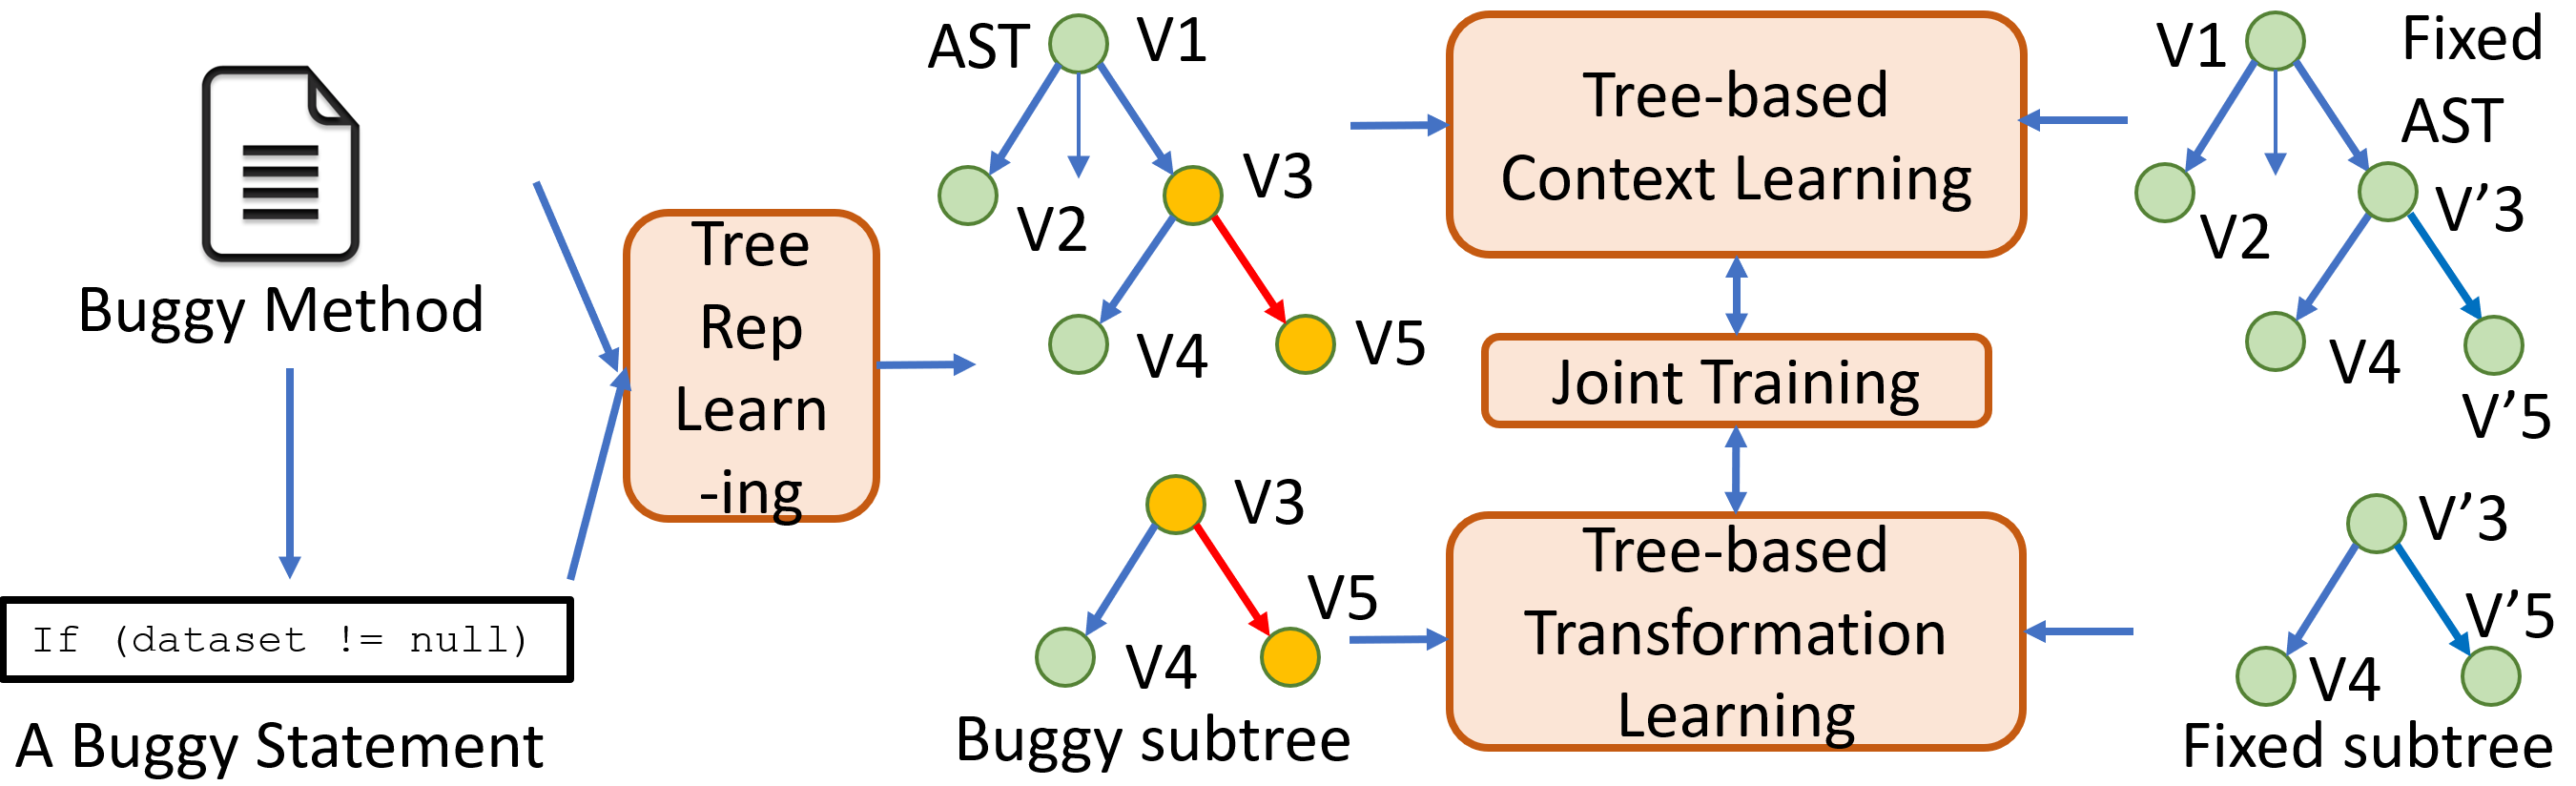
\includegraphics[width=3.4in]{graphs/overview-training.png}
	\caption{{\tool}: Training}
	\label{overview-training}
\end{figure}

\noindent {\bf Tree-based Representation Learning.} The goal of this
step is to take the source code under study and to build the
tree-based vector representations (embeddings) to be the input for our
dual models: \code{CCL} and \code{CTL}. To achieve that, we first
parse the given source code to obtain the abstract syntax tree (AST)
for the entire method and the subtree for the buggy statement.  We
then use a word embedding technique to produce the vector for each
node in the AST when we flatten the AST. The output of this step is
the AST for the method and the AST subtree for the buggy statement in
which each node is replaced by its embedding vector
(Figure~\ref{overview-training}).

\noindent {\bf Context-aware Dual Learning Automated Program Repair.}
The goal of this step is to train both of the tree-based context
learning model (\code{CCL}) and the tree-based code transformation
mdeol (\code{CTL}) at the joint training manner. The entire AST of the
buggy method after vectorization (i.e., each node is a vector) is used
at the input layer of the context learning model (\code{CCL}) for
training. The AST of the corresponding fixed method after
vectorization is used at the output layer of the \code{CCL}
model. Similarly, the AST subtree of the buggy statement after
vectorization is used at the input layer of the transformation
learning model (\code{CTL}), and the subtree of the fixed statement
after vectorization is used at the output layer of the \code{CTL}
model. Each of the CCL and CTL models is realized via an
attention-based \code{seq2seq} model~\cite{yi}. Instead of cascading
the two models \code{CCL} and \code{CTL}, we use a mechanism called
{\em cross-stitch unit}~\cite{misra2016cross}, to train them
simultaneously with soft-sharing the parameters to exploit this
duality. The sharing of representations between \code{CCL} amd
\code{CTL} is modeled by learning a linear combination of the input
features in both models. The output of this step includes the trained
\code{CCL} and \code{CTL} models.

\subsection{Prediction Process}

\begin{figure}[t]
	\centering
	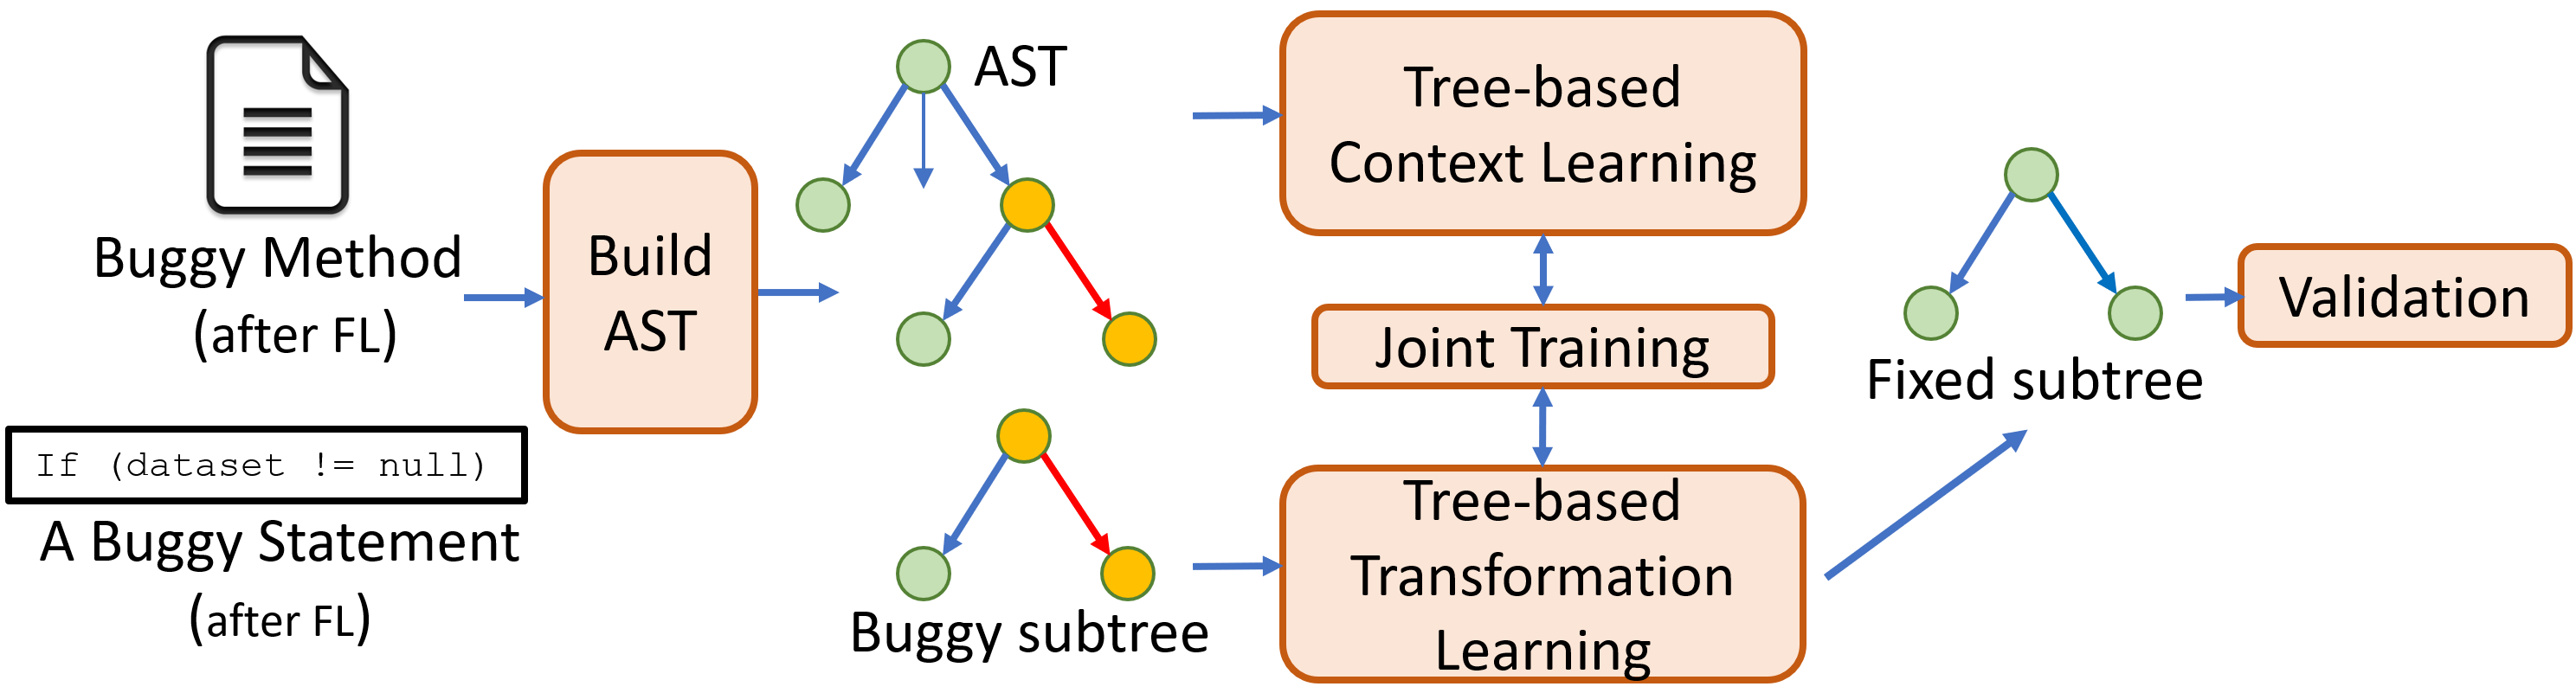
\includegraphics[width=3.4in]{graphs/overview-predict.png}
	\caption{{\tool}: Fixing}
	\label{overview-fixing}
\end{figure}

Figure~\ref{overview-fixing} illustrates the prediction, i.e., the
automated fixing process. 
